\section{Evaluation}
\label{cp5:evaluation}


Our evaluation focuses 
on determining what portion of the text identified by human annotators the techniques that we explore can automatically identify.
Our experimental setup is as follows.



\subsubsection{Metrics}


Ultimately, the goal of our evaluation is to assist the design of tools that help developers quickly locate the text relevant to their tasks, surfacing or highlighting the identified text in an artifact under inspection~\cite{Robillard2015}.
This means that the text identified by a technique represents a set containing the information to be surfaced and thus, 
we use \textit{precision} and \textit{recall} to measure the accuracy of each technique~\cite{Manning2009IR}.
We use the evaluation outcomes detailed in Table~\ref{tbl:type-I-II-errors} to understand each metric.

\medskip
\begin{table}[H]
\centering    
\begin{scriptsize}
\begin{threeparttable}
\begin{tabular}{l|l|l}

\hline

\textbf{}
& \textbf{Relevant}    
& \textbf{Not-relevant} \\

\hline

\textbf{Identified as relevant} & true positive ($TP$) & false positive ($FP$) \\
\hline
\textbf{Identified as Not-relevant} & false negative ($FN$) & true negative ($TN$) \\
\hline

\end{tabular}
\end{threeparttable}
\end{scriptsize}
\caption{Evaluation outcomes}
\label{tbl:type-I-II-errors}
\end{table}

    



\paragraph{\textbf{Precision}}

Precision measures the fraction of the sentences identified that are relevant over the total number of sentences identified, as shown in Equation~\ref{eq:cp5:precision}.



\begin{equation}
\label{eq:cp5:precision}    
    Precision = \frac{TP}{TP + FP}
\end{equation}


\paragraph{\textbf{Recall}} Recall represents how many of all marked sentences are identified by a technique (Equation~\ref{eq:cp5:recall}).


\begin{equation}
\label{eq:cp5:recall}        
    Recall = \frac{TP}{TP + FN}
\end{equation}



\paragraph{\textbf{Pyramid Precision \& Pyramid Recall}} 

We measure precision and recall considering sentences marked by two or more annotators; this, however ignores the fact that text marked by a single annotator can equally contribute towards task completion~\cite{marques2020}. To address the text identified by a single annotator, we 
follow evaluation procedures outlined by Lotufo et al.~\cite{Lotufo2012} and we
also report pyramid precision and pyramid recall. These metrics are similar to the ones defined in 
Equations~\ref{eq:cp5:precision} and~\ref{eq:cp5:recall} but treat any of the text marked as relevant.






\subsubsection{Baseline}


As done by~\cite{Lin2021} and~\cite{Ye2016}, we use a standard VSM lexical similarity approach as a baseline. Our rationale to use 
lexical similarity is based on the fact that 
both our card sorting analysis (\red{Chapter~\ref{aaa}}) and related work~\cite{Ko2006a, Freund2015} has shown that developers often use keyword-matching as a simple and quick search strategy to locate text that might contain information relevant to their tasks.


Following procedures analogous to the semantic similarity-based technique (Section~\ref{cp5:approach-w2v}), we compute lexical similarity and output the top-n sentences with highest similarity as the ones likely relevant to an input software task.




\subsubsection{Techniques Configuration}


\art{I could move this section to a subsection or a paragraph at the end of each technique in Section~\ref{cp5:approaches}}


Both the \texttt{baseline} and the \texttt{word2vec} techniques have a set number of sentences in the techniques output. To determine how many sentences these approaches should output, we consider that 
no more than 20\% of the content in the corpora are deemed relevant to a task, which, on average, accounts for 8.93 sentences (\red{Chapter~\ref{}}). We approximate these values to identifying a target number of 10 sentences per input task-artifact, a value that will also allow us to compare the accuracy of our approach to previous work with similar experimental setup, e.g., ~\cite{Xu2017} or~\cite{Lotufo2012}.




% For this evaluation, we set the target number of sentences identified (i.e., length of a summary) to 20\% of the content of an artifact,
% which is a value derived from our study on characterizing 
% task-relevant information in natural language artifacts~\cite{marques2020}.




For the BERT technique, we fine-tune the model training it for up to 10 epochs with a \textit{batch size}---the number of samples passed through the model network at once---of 64. Since the sentences in a task and software artifact are fairly short, with an average length of 26 tokens, we also set the model's sequence length to 64. Cross Entropy is our loss function, and the model is trained to minimize it using the Adam optimizer at a learning rate of \textit{1e-5} with an early stopping criterion. As for training data, we explore two configurations:


\boldparagraph{BERT\textsubscript{DS-android}}{
We split the data available in the \acs{DS-android} dataset and use part of it for training. 
As done by other studies (e.g.,~\cite{Chaparro2017, fucci2019, Petrosyan2015}), we use standard cross-validation techniques to ensure  that no data used for evaluation, i.e., testing, is also used
during the model's training procedures, i.e., training and validation. More specifically, we use 10-fold cross-validation with 70\%, 20\% and 10\% splits for training, validation and testing. \red{ref} We refer to this configuration as \texttt{BERT\textsubscript{DS-android}}.
}

\boldparagraph{BERT\textsubscript{DS-synthetic}}{
To study the impacts of training data on BERT, we train the model in a smaller dataset containing six tasks and a total of 1874 sentences, from which 602 of them were deemed relevant by 20 participants with software development experience (\red{Chapter~\ref{aaa}}). The tasks in this dataset were not drawn from open-source systems, but rather created to stimulate the participants' information-seeking behaviour. Due to the synthetic nature of the tasks in this dataset, we refer to this configuration as \texttt{BERT\textsubscript{DS-synthetic}}.
}

\clearpage

\subsection{Results}



We have a total of 1393 sentences marked as relevant by human annotators. When compared to the text automatically identified by each approach,
we observe that the baseline approach identifies, \texttt{VSM}, identifies \red{112} sentences while word2vec indentifies 







\begin{table}[H]
\centering    
\begin{small}
\begin{threeparttable}
\begin{tabular}{lccccc}


\textbf{technique} & 
\textbf{precision} & \textbf{recall} & 
$\Delta$ \textbf{precision} & $\Delta$ \textbf{recall} \\


\hline


\texttt{baseline} &
0.30 & 0.33 &  
0.38 & 0.48 
\\

\texttt{word2vec + association-pairs} &
0.52 & 0.53 &  
0.52 & 0.51
\\

% \texttt{BERT\textsubscript{DS-synthetic}} &
% 0.54 & 0.55 & 0.51 & 
% 0.55 & 0.57 
% \\

\texttt{BERT\textsubscript{DS-android} + frame-elements} &
0.55 & 0.56 & 
0.55 & 0.56 
\\

\hline

\end{tabular}
\end{threeparttable}
\end{small}
\caption{Pyramid precision, pyramid recall comparison}
\label{tbl:approach-results-overall}
\end{table}








\begin{figure}
    \centering
    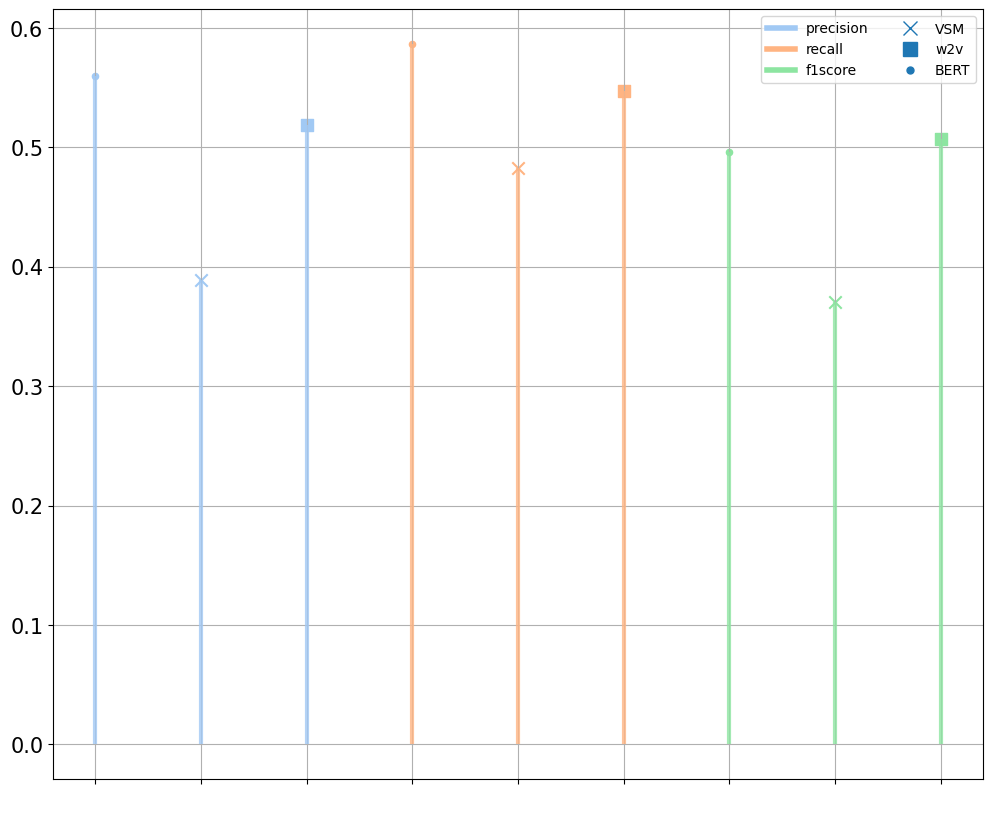
\includegraphics[width=0.95\textwidth]{cp5/results_lollipop}
    \caption{Evaluation results for each technique configuration \red{Draft: I will split the figure in 3. One for each metric. The markers will represent the filters}}
    % \label{fig:webview-task}
\end{figure}







% \art{Change from tables to plots. Similar to Sarah and Treude~\cite{nadi2020}, show Venn diagram with how many sentences each approach identifies and overlaps between them}
\art{Consider changing from tables to plots.}


% \begin{table}[H]
\centering    
\begin{small}
\begin{threeparttable}
\begin{tabular}{lcccc}


\textbf{Technique} & 
\textbf{Precision} & \textbf{Recall} & 
\parbox[c][.9cm][c]{1.5cm}{\centering \textbf{Pyramid precision}} & 
\parbox[c][.9cm][c]{1.5cm}{\centering \textbf{Pyramid recall}} \\


\hline


\textbf{word2vec + meaningful-frames} &
0.50 & 0.50 & 
0.50 & 0.50 
\\

\textbf{word2vec + similar-meaning} &
0.50 & 0.50 & 
0.50 & 0.50 
\\


\textbf{BERT + meaningful-frames} &
0.50 & 0.50 & 
0.50 & 0.50 
\\

\textbf{BERT + meaningful-frames} &
0.50 & 0.50 & 
0.50 & 0.50 
\\

\hline

\end{tabular}
\end{threeparttable}
\end{small}
\caption{\art{this can be merged with the previous table}}
\end{table}




% \begin{table}[H]
\centering    
\begin{scriptsize}
\begin{threeparttable}
\begin{tabular}{llcccc}


\textbf{} & \textbf{Technique} &
\textbf{Precision} & \textbf{Recall} & 
\parbox[c][.7cm][c]{1.5cm}{\centering \textbf{Pyramid precision}} & 
\parbox[c][.7cm][c]{1.5cm}{\centering \textbf{Pyramid recall}} \\


\hline

\multirow{ 2}{*}{\textbf{Baseline}}  & VSM &
0.50 & 0.50 & 
0.50 & 0.50 
\\

& ours &
0.50 & 0.50 & 
0.50 & 0.50 
\\

\hline

\multirow{ 2}{*}{\textbf{API documentation}}  & Kreck &
0.50 & 0.50 & 
0.50 & 0.50 
\\

& ours &
0.50 & 0.50 & 
0.50 & 0.50 
\\

\hline

\multirow{ 2}{*}{\textbf{GitHub issues}} & Hurried &
0.50 & 0.50 & 
0.50 & 0.50 
\\

 & Ours &
0.50 & 0.50 & 
0.50 & 0.50 
\\

\hline

\multirow{ 2}{*}{\textbf{SO answers}} & AnsBot &
0.50 & 0.50 & 
0.50 & 0.50 
\\

 & Ours &
0.50 & 0.50 & 
0.50 & 0.50 
\\

\hline

\end{tabular}
\end{threeparttable}
\end{scriptsize}
\caption{Techniques comparison}
\label{tbl:approach-results-artifacts}
\end{table}








